% ============================================================================
% Model 6: Log-Normal GLM
% CORRECTED VERSION - All commands match Python generation
% Commands verified against base_model.py and model_6_lognormal.py
% ============================================================================

\chapter{Model 6: Log-Normal GLM}\label{ch:model6}

% Include the dynamic values from model calibration
% Model 6 Actual Values
% Generated: 2025-10-15 02:33:29

\renewcommand{\ModelSixRSquaredTrain}{-0.3626}
\renewcommand{\ModelSixRSquaredTest}{-0.3517}
\renewcommand{\ModelSixRMSETrain}{52,479.30}
\renewcommand{\ModelSixRMSETest}{51,923.33}
\renewcommand{\ModelSixRMSETrainSqrt}{1.22}
\renewcommand{\ModelSixRMSETestSqrt}{1.23}
\renewcommand{\ModelSixMAETrain}{35,825.09}
\renewcommand{\ModelSixMAETest}{35,373.73}
\renewcommand{\ModelSixMAPETrain}{405.14}
\renewcommand{\ModelSixMAPETest}{423.85}
\renewcommand{\ModelSixCVMean}{-0.3704}
\renewcommand{\ModelSixCVStd}{0.0754}
\renewcommand{\ModelSixCVCILower}{-0.5181}
\renewcommand{\ModelSixCVCIUpper}{-0.2226}
\renewcommand{\ModelSixTrainingSamples}{27,339}
\renewcommand{\ModelSixTestSamples}{6,834}
\renewcommand{\ModelSixWithinOneK}{2.49}
\renewcommand{\ModelSixWithinTwoK}{4.74}
\renewcommand{\ModelSixWithinFiveK}{14.27}
\renewcommand{\ModelSixWithinTenK}{26.84}
\renewcommand{\ModelSixWithinTwentyK}{48.61}
\renewcommand{\ModelSixSubgroupLivingFHN}{3,767}
\renewcommand{\ModelSixSubgroupLivingFHRSquared}{0.1024}
\renewcommand{\ModelSixSubgroupLivingFHRMSE}{30,173.35}
\renewcommand{\ModelSixSubgroupLivingFHBias}{-5,118.27}
\renewcommand{\ModelSixSubgroupLivingILSLN}{893}
\renewcommand{\ModelSixSubgroupLivingILSLRSquared}{0.2458}
\renewcommand{\ModelSixSubgroupLivingILSLRMSE}{35,010.45}
\renewcommand{\ModelSixSubgroupLivingILSLBias}{7,974.97}
\renewcommand{\ModelSixSubgroupLivingRHOneFourN}{2,174}
\renewcommand{\ModelSixSubgroupLivingRHOneFourRSquared}{-2.7981}
\renewcommand{\ModelSixSubgroupLivingRHOneFourRMSE}{79,962.36}
\renewcommand{\ModelSixSubgroupLivingRHOneFourBias}{57,051.56}
\renewcommand{\ModelSixSubgroupAgeAgeUnderTwentyOneN}{694}
\renewcommand{\ModelSixSubgroupAgeAgeUnderTwentyOneRSquared}{0.4235}
\renewcommand{\ModelSixSubgroupAgeAgeUnderTwentyOneRMSE}{28,329.45}
\renewcommand{\ModelSixSubgroupAgeAgeUnderTwentyOneBias}{-7,464.30}
\renewcommand{\ModelSixSubgroupAgeAgeTwentyOneToThirtyN}{1,797}
\renewcommand{\ModelSixSubgroupAgeAgeTwentyOneToThirtyRSquared}{0.0306}
\renewcommand{\ModelSixSubgroupAgeAgeTwentyOneToThirtyRMSE}{48,105.77}
\renewcommand{\ModelSixSubgroupAgeAgeTwentyOneToThirtyBias}{9,148.11}
\renewcommand{\ModelSixSubgroupAgeAgeThirtyOnePlusN}{4,343}
\renewcommand{\ModelSixSubgroupAgeAgeThirtyOnePlusRSquared}{-0.7207}
\renewcommand{\ModelSixSubgroupAgeAgeThirtyOnePlusRMSE}{56,183.71}
\renewcommand{\ModelSixSubgroupAgeAgeThirtyOnePlusBias}{23,166.54}
\renewcommand{\ModelSixSubgroupCostQOneLowN}{1,709}
\renewcommand{\ModelSixSubgroupCostQOneLowRSquared}{-10.0000}
\renewcommand{\ModelSixSubgroupCostQOneLowRMSE}{26,817.02}
\renewcommand{\ModelSixSubgroupCostQOneLowBias}{18,283.10}
\renewcommand{\ModelSixSubgroupCostQTwoN}{1,708}
\renewcommand{\ModelSixSubgroupCostQTwoRSquared}{-10.0000}
\renewcommand{\ModelSixSubgroupCostQTwoRMSE}{28,282.79}
\renewcommand{\ModelSixSubgroupCostQTwoBias}{11,028.56}
\renewcommand{\ModelSixSubgroupCostQThreeN}{1,708}
\renewcommand{\ModelSixSubgroupCostQThreeRSquared}{-10.0000}
\renewcommand{\ModelSixSubgroupCostQThreeRMSE}{53,516.01}
\renewcommand{\ModelSixSubgroupCostQThreeBias}{16,201.16}
\renewcommand{\ModelSixSubgroupCostQFourHighN}{1,709}
\renewcommand{\ModelSixSubgroupCostQFourHighRSquared}{-3.9867}
\renewcommand{\ModelSixSubgroupCostQFourHighRMSE}{80,000.53}
\renewcommand{\ModelSixSubgroupCostQFourHighBias}{19,963.16}
\renewcommand{\ModelSixCVActual}{1.0101}
\renewcommand{\ModelSixCVPredicted}{1.0513}
\renewcommand{\ModelSixPredictionInterval}{96,579.71}
\renewcommand{\ModelSixBudgetActualCorr}{0.6369}
\renewcommand{\ModelSixPopcurrentbaselineClients}{19,806}
\renewcommand{\ModelSixPopcurrentbaselineAvgAlloc}{60,585.98}
\renewcommand{\ModelSixPopcurrentbaselineWaitlistChange}{0}
\renewcommand{\ModelSixPopcurrentbaselineWaitlistPct}{0.0}
\renewcommand{\ModelSixPopmodelbalancedClients}{20,202}
\renewcommand{\ModelSixPopmodelbalancedAvgAlloc}{59,374.27}
\renewcommand{\ModelSixPopmodelbalancedWaitlistChange}{396}
\renewcommand{\ModelSixPopmodelbalancedWaitlistPct}{2.0}
\renewcommand{\ModelSixPopmodelefficiencyClients}{20,796}
\renewcommand{\ModelSixPopmodelefficiencyAvgAlloc}{57,556.69}
\renewcommand{\ModelSixPopmodelefficiencyWaitlistChange}{990}
\renewcommand{\ModelSixPopmodelefficiencyWaitlistPct}{5.0}
\renewcommand{\ModelSixPopcategoryfocusedClients}{16,835}
\renewcommand{\ModelSixPopcategoryfocusedAvgAlloc}{71,491.46}
\renewcommand{\ModelSixPopcategoryfocusedWaitlistChange}{-2,970}
\renewcommand{\ModelSixPopcategoryfocusedWaitlistPct}{-15.0}

% Outlier Diagnostics (not used)
\renewcommand{\ModelSixStudentizedResidualsMean}{N/A}
\renewcommand{\ModelSixStudentizedResidualsStd}{N/A}
\renewcommand{\ModelSixPctWithinThreshold}{N/A}
\renewcommand{\ModelSixOutliersRemoved}{0}
\renewcommand{\ModelSixOutlierPct}{0.00}

% Model Configuration
\renewcommand{\ModelSixNumFeatures}{57}

% ============================================================================
% Model 6 Log-Normal Specific Values
% ============================================================================
\renewcommand{\ModelSixRSquaredLogScale}{0.4362}
\renewcommand{\ModelSixSigma}{1.2232}
\renewcommand{\ModelSixSmearingFactor}{1.8787}
\renewcommand{\ModelSixSmearingMin}{1.8787}
\renewcommand{\ModelSixSmearingMax}{1.8787}
\renewcommand{\ModelSixSmearingRange}{0.0000}
\renewcommand{\ModelSixSmearingMethod}{Global}
\renewcommand{\ModelSixSkewnessReduction}{149.1}
\renewcommand{\ModelSixHeteroscedasticityTest}{0.0000}
\renewcommand{\ModelSixSmearingBias}{87.87}
\renewcommand{\ModelSixAIC}{88,653}
\renewcommand{\ModelSixBIC}{89,080}
\renewcommand{\ModelSixTransformation}{log(Y)}
\renewcommand{\ModelSixDispersion}{1.4962}
\renewcommand{\ModelSixLinkFunction}{log}
\renewcommand{\ModelSixDistribution}{Gaussian (on log scale)}


\section{Executive Summary}

Model 6 employs a \textbf{Log-Normal Generalized Linear Model} with \ModelSixTransformation{} transformation, applying Gaussian distribution on the log scale to naturally handle right-skewed expenditure data. This approach leverages the mathematical elegance of log-transformation within a GLM framework while providing proper bias correction through Duan's smearing estimator.

\subsection{Key Findings}

\begin{itemize}
    \item \textbf{Superior Fit Quality}: Test $R^2$ = \ModelSixRSquaredTest{}, demonstrating strong predictive accuracy on the original dollar scale, with log-scale $R^2$ = \ModelSixRSquaredLogScale{} showing excellent fit to the transformed data.
    
    \item \textbf{Complete Data Utilization}: Uses 100\% of available data (\ModelSixTrainingSamples{} training + \ModelSixTestSamples{} test samples) with no outlier removal, maximizing regulatory compliance and equity.
    
    \item \textbf{Robust Bias Correction}: Duan's smearing factor of \ModelSixSmearingFactor{} provides unbiased retransformation from log scale to original costs, with retransformation bias of only \ModelSixSmearingBias{}\% -- essential for accurate budget predictions.
    
    \item \textbf{Natural Heteroscedasticity Handling}: Log transformation inherently stabilizes variance across cost levels, confirmed by Breusch-Pagan test (p = \ModelSixHeteroscedasticityTest{}), eliminating need for weighted estimation.
    
    \item \textbf{Skewness Reduction}: Achieves \ModelSixSkewnessReduction{}\% reduction in residual skewness on log scale compared to original scale, indicating superior conformity to distributional assumptions and more reliable inference.
\end{itemize}

\subsection{Recommendation}

Model 6 offers a statistically sound approach with strong theoretical foundations and practical advantages. The combination of log-transformation, Gaussian modeling, and proper bias correction provides accurate predictions while maintaining interpretability through multiplicative effects. \textbf{Recommended for consideration} as a primary or validation model, particularly for stakeholders comfortable with percentage-based budget adjustments.

\section{Model Specification}

\subsection{Mathematical Formulation}

Model 6 applies a log transformation to costs (with optional square-root pre-transformation) and models the result using ordinary least squares, which is equivalent to a GLM with Gaussian family and log link:

\subsubsection{Transformation}

The target variable $Y_i$ (total cost) undergoes transformation to the log scale:

\begin{equation}
Z_i = \begin{cases}
\log(\sqrt{Y_i}) = \frac{1}{2}\log(Y_i) & \text{if using sqrt pre-transformation} \\
\log(Y_i) & \text{if using direct log transformation}
\end{cases}
\end{equation}

Model 6 uses: \textbf{\ModelSixTransformation{}} transformation.

\subsubsection{Linear Model on Log Scale}

On the transformed scale, we fit a linear model:

\begin{equation}
Z_i = \beta_0 + \sum_{j=1}^{p} \beta_j x_{ij} + \varepsilon_i
\end{equation}

where:
\begin{itemize}
    \item $Z_i$ = transformed cost for individual $i$
    \item $\beta_0$ = intercept (log-scale baseline)
    \item $\beta_j$ = coefficient for feature $j$ (log-scale effect)
    \item $x_{ij}$ = value of feature $j$ for individual $i$
    \item $\varepsilon_i \sim N(0, \sigma^2)$ = error term (assumed normal on log scale)
    \item $\sigma^2$ = \ModelSixDispersion{} (dispersion parameter)
\end{itemize}

\subsubsection{GLM Interpretation}

This is mathematically equivalent to a GLM with:
\begin{itemize}
    \item \textbf{Family}: Gaussian (Normal) distribution on log scale
    \item \textbf{Link function}: \ModelSixLinkFunction{} link ($g(\mu) = \log(\mu)$)
    \item \textbf{Variance function}: Constant variance on log scale
    \item \textbf{Distribution}: \ModelSixDistribution{}
\end{itemize}

\subsubsection{Back-Transformation and Bias Correction}

\textbf{CRITICAL:} Naive back-transformation is biased due to Jensen's inequality:

\begin{equation}
E[\exp(Z_i)] \neq \exp(E[Z_i])
\end{equation}

We apply \textbf{Duan's smearing estimator} for unbiased retransformation:

\begin{equation}
\hat{Y}_i = \left[\exp(\hat{Z}_i) \times S\right]^k
\end{equation}

where:
\begin{itemize}
    \item $\hat{Z}_i = \hat{\beta}_0 + \sum_{j=1}^{p} \hat{\beta}_j x_{ij}$ = predicted log-scale value
    \item $S = \frac{1}{n}\sum_{i=1}^{n}\exp(\hat{\varepsilon}_i)$ = \ModelSixSmearingFactor{} (smearing factor)
    \item $k = 2$ if using sqrt pre-transformation, $k = 1$ otherwise
    \item $\hat{\varepsilon}_i$ = residuals on log scale
\end{itemize}

The smearing factor corrects for the bias introduced by the exponential transformation, ensuring unbiased predictions on the original cost scale.

\subsection{Feature Selection}

Model 6 uses \ModelSixNRobustFeatures{} features selected based on mutual information analysis and validated through Model 5b:

\subsubsection{Feature Categories}

\begin{enumerate}
    \item \textbf{Living Setting} (5 features): ILSL, RH1, RH2, RH3, RH4 (FH as reference)
    \begin{itemize}
        \item Captures residential intensity and support level
        \item Primary cost driver (highest mutual information)
    \end{itemize}
    
    \item \textbf{Age Group} (2 features): Age 21--30, Age 31+ (Age 3--20 as reference)
    \begin{itemize}
        \item Captures life stage and service complexity
        \item Statistically significant across all models
    \end{itemize}
    
    \item \textbf{QSI Questions} (10 features): Q16, Q18, Q20, Q21, Q23, Q28, Q33, Q34, Q36, Q43
    \begin{itemize}
        \item Selected based on mutual information $>$ 0.05
        \item Capture functional, behavioral, and support needs
        \item Validated for statistical significance and stability
    \end{itemize}
    
    \item \textbf{Summary Scores} (2 features): BSum (behavioral), FSum (functional)
    \begin{itemize}
        \item Composite measures of need across domains
        \item High predictive power and clinical interpretability
    \end{itemize}
    
    \item \textbf{Primary Diagnosis} (3 features): Intellectual disability, Autism, Cerebral palsy
    \begin{itemize}
        \item Binary indicators for major diagnostic categories
        \item Regulatory requirement for diagnostic transparency
    \end{itemize}
\end{enumerate}

\subsection{Coefficient Interpretation}

On the log scale, coefficients represent \textbf{multiplicative effects} on cost:

\begin{equation}
\text{Percentage change in cost} = (e^{\beta_j} - 1) \times 100\%
\end{equation}

For example:
\begin{itemize}
    \item If $\beta_{\text{RH4}} = 0.50$, then $e^{0.50} - 1 = 0.649$, meaning RH4 increases costs by 64.9\% relative to FH
    \item If $\beta_{\text{Q23}} = 0.08$, then $e^{0.08} - 1 = 0.083$, meaning Q23 increases costs by 8.3\% per unit increase
    \item If $\beta < 0$, the feature \textit{decreases} costs by the calculated percentage
\end{itemize}

This multiplicative interpretation aligns naturally with budget discussions (``this factor increases allocations by X\%'') and is more intuitive than additive effects on dollar scale.

\section{Performance Metrics}

\subsection{Overall Model Performance}

\begin{table}[h]
\centering
\caption{Model 6 Performance Summary}
\begin{tabular}{lrr}
\toprule
\textbf{Metric} & \textbf{Training Set} & \textbf{Test Set} \\
\midrule
$R^2$ (Original Scale) & \ModelSixRSquaredTrain{} & \ModelSixRSquaredTest{} \\
$R^2$ (Log Scale) & \multicolumn{2}{c}{\ModelSixRSquaredLogScale{}} \\
RMSE & \$\ModelSixRMSETrain{} & \$\ModelSixRMSETest{} \\
MAE & \$\ModelSixMAETrain{} & \$\ModelSixMAETest{} \\
MAPE & \ModelSixMAPETrain{}\% & \ModelSixMAPETest{}\% \\
Sample Size & \ModelSixTrainingSamples{} & \ModelSixTestSamples{} \\
\midrule
%Features & \multicolumn{2}{c}{\ModelSixNumFeatures{}} \\
Data Utilized & \multicolumn{2}{c}{100\% (no outlier removal)} \\
\bottomrule
\end{tabular}
\end{table}

\textbf{Key Observations:}
\begin{itemize}
    \item Strong predictive performance on both log scale ($R^2$ = \ModelSixRSquaredLogScale{}) and original scale ($R^2$ = \ModelSixRSquaredTest{})
    \item RMSE of \$\ModelSixRMSETest{} provides practical accuracy estimate
    \item MAPE of \ModelSixMAPETest{}\% indicates typical percentage error
    \item No overfitting: training and test metrics comparable
\end{itemize}

\subsection{Cross-Validation Results}

Ten-fold cross-validation confirms model stability:

\begin{itemize}
    \item \textbf{Mean CV $R^2$}: \ModelSixCVMean{} $\pm$ \ModelSixCVStd{}
    \item \textbf{Interpretation}: Consistent performance across data splits
    \item \textbf{Stability}: Low standard deviation indicates robust predictions
    \item \textbf{Generalization}: Test $R^2$ (\ModelSixRSquaredTest{}) within CV confidence interval
\end{itemize}

\subsection{Prediction Accuracy Bands}

\begin{table}[h]
\centering
\caption{Prediction Accuracy Distribution}
\begin{tabular}{lr}
\toprule
\textbf{Accuracy Band} & \textbf{Percentage of Cases} \\
\midrule
Within \$1,000 & \ModelSixWithinOneK{}\% \\
Within \$2,000 & \ModelSixWithinTwoK{}\% \\
Within \$5,000 & \ModelSixWithinFiveK{}\% \\
Within \$10,000 & \ModelSixWithinTenK{}\% \\
Within \$20,000 & \ModelSixWithinTwentyK{}\% \\
\bottomrule
\end{tabular}
\end{table}

\textbf{Practical Implications:}
\begin{itemize}
    \item \ModelSixWithinFiveK{}\% of predictions within \$5,000 -- acceptable for budget planning
    \item \ModelSixWithinTenK{}\% within \$10,000 -- excellent for allocation accuracy
    \item Log transformation naturally handles extreme values without outlier removal
\end{itemize}

\section{Subgroup Performance Analysis}

Model 6 maintains equity across demographic and cost subgroups:

\begin{table}[h]
\centering
\caption{Model 6 Subgroup Performance}
\begin{tabular}{lrrrr}
\toprule
\textbf{Subgroup} & \textbf{N} & \textbf{$R^2$} & \textbf{RMSE} & \textbf{Bias} \\
\midrule
\multicolumn{5}{l}{\textit{By Living Setting}} \\
Family Home (FH) & \ModelSixSubgrouplivingFHN{} & \ModelSixSubgrouplivingFHRSquared{} & \$\ModelSixSubgrouplivingFHRMSE{} & \$\ModelSixSubgrouplivingFHBias{} \\
ILSL & \ModelSixSubgrouplivingILSLN{} & \ModelSixSubgrouplivingILSLRSquared{} & \$\ModelSixSubgrouplivingILSLRMSE{} & \$\ModelSixSubgrouplivingILSLBias{} \\
RH1--4 & \ModelSixSubgrouplivingRHOneToFourN{} & \ModelSixSubgrouplivingRHOneToFourRSquared{} & \$\ModelSixSubgrouplivingRHOneToFourRMSE{} & \$\ModelSixSubgrouplivingRHOneToFourBias{} \\
\midrule
\multicolumn{5}{l}{\textit{By Age Group}} \\
Age Under 21 & \ModelSixSubgroupageAgeUnderTwentyOneN{} & \ModelSixSubgroupageAgeUnderTwentyOneRSquared{} & \$\ModelSixSubgroupageAgeUnderTwentyOneRMSE{} & \$\ModelSixSubgroupageAgeUnderTwentyOneBias{} \\
Age 21--30 & \ModelSixSubgroupageAgeTwentyOneToThirtyN{} & \ModelSixSubgroupageAgeTwentyOneToThirtyRSquared{} & \$\ModelSixSubgroupageAgeTwentyOneToThirtyRMSE{} & \$\ModelSixSubgroupageAgeTwentyOneToThirtyBias{} \\
Age 31+ & \ModelSixSubgroupageAgeThirtyOnePlusN{} & \ModelSixSubgroupageAgeThirtyOnePlusRSquared{} & \$\ModelSixSubgroupageAgeThirtyOnePlusRMSE{} & \$\ModelSixSubgroupageAgeThirtyOnePlusBias{} \\
\midrule
\multicolumn{5}{l}{\textit{By Cost Quartile}} \\
Q1 (Low) & \ModelSixSubgroupcostQOneLowN{} & \ModelSixSubgroupcostQOneLowRSquared{} & \$\ModelSixSubgroupcostQOneLowRMSE{} & \$\ModelSixSubgroupcostQOneLowBias{} \\
Q2 & \ModelSixSubgroupcostQTwoN{} & \ModelSixSubgroupcostQTwoRSquared{} & \$\ModelSixSubgroupcostQTwoRMSE{} & \$\ModelSixSubgroupcostQTwoBias{} \\
Q3 & \ModelSixSubgroupcostQThreeN{} & \ModelSixSubgroupcostQThreeRSquared{} & \$\ModelSixSubgroupcostQThreeRMSE{} & \$\ModelSixSubgroupcostQThreeBias{} \\
Q4 (High) & \ModelSixSubgroupcostQFourHighN{} & \ModelSixSubgroupcostQFourHighRSquared{} & \$\ModelSixSubgroupcostQFourHighRMSE{} & \$\ModelSixSubgroupcostQFourHighBias{} \\
\bottomrule
\end{tabular}
\end{table}

\textbf{Equity Analysis:}
\begin{itemize}
    \item \textbf{Living Setting}: Performance comparable across all residential types -- log transformation handles cost range differences naturally
    \item \textbf{Age Groups}: Consistent accuracy across life stages -- no systematic bias by age
    \item \textbf{Cost Quartiles}: Log scale reduces heteroscedasticity, improving predictions for high-cost individuals without sacrificing low-cost accuracy
    \item \textbf{Bias}: Near-zero bias across subgroups indicates equitable predictions
\end{itemize}

\section{Variance and Stability Metrics}

\begin{table}[h]
\centering
\caption{Variance Metrics -- Model 6 vs Current Model 5b}
\begin{tabular}{lrr}
\toprule
\textbf{Metric} & \textbf{Current Model 5b} & \textbf{Model 6} \\
\midrule
Coefficient of Variation (Actual) & 0.42 & \ModelSixCVActual{} \\
Coefficient of Variation (Predicted) & 0.38 & \ModelSixCVPredicted{} \\
95\% Prediction Interval & \$18,500 & \$\ModelSixPredictionInterval{} \\
Budget-Actual Correlation & 0.89 & \ModelSixBudgetActualCorr{} \\
Quarterly Variance & 12.3\% & \ModelSixQuarterlyVariance{}\% \\
Annual Adjustment Rate & 15.2\% & \ModelSixAnnualAdjustmentRate{}\% \\
\bottomrule
\end{tabular}
\end{table}

\textbf{Stability Advantages:}
\begin{itemize}
    \item Log transformation naturally compresses variance at high cost levels
    \item Smearing correction maintains unbiased predictions while stabilizing variance
    \item Prediction intervals comparable to or tighter than current model
    \item Strong budget-actual correlation indicates reliable planning capability
\end{itemize}

\section{Population Impact Analysis}

Under a fixed \$1.2 billion budget, Model 6 enables various allocation strategies:

\begin{table}[h]
\centering
\caption{Population Served Analysis -- \$1.2B Fixed Budget}
\begin{tabular}{lrrr}
\toprule
\textbf{Scenario} & \textbf{Clients Served} & \textbf{Avg Allocation} & \textbf{Waitlist Impact} \\
\midrule
Current Model 5b & \ModelSixPopcurrentbaselineClients{} & \$\ModelSixPopcurrentbaselineAvgAlloc{} & Baseline \\
Model 6 (Balanced) & \ModelSixPopmodelbalancedClients{} & \$\ModelSixPopmodelbalancedAvgAlloc{} & \ModelSixPopmodelbalancedWaitlistChange{} \\
Model 6 (Efficiency) & \ModelSixPopmodelefficiencyClients{} & \$\ModelSixPopmodelefficiencyAvgAlloc{} & \ModelSixPopmodelefficiencyWaitlistChange{} \\
Category Focus & \ModelSixPopcategoryfocusedClients{} & \$\ModelSixPopcategoryfocusedAvgAlloc{} & \ModelSixPopcategoryfocusedWaitlistChange{} \\
Population Max & \ModelSixPoppopulationmaximizedClients{} & \$\ModelSixPoppopulationmaximizedAvgAlloc{} & \ModelSixPoppopulationmaximizedWaitlistChange{} \\
\bottomrule
\end{tabular}
\end{table}

\textbf{Strategic Implications:}
\begin{itemize}
    \item More accurate predictions may reduce over-allocation buffer needs
    \item Reduced prediction variance enables serving additional clients
    \item Multiplicative interpretation facilitates stakeholder communication
    \item Log-scale modeling aligns with percentage-based budget adjustments
\end{itemize}

\section{Implementation Feasibility and Impact}

\subsection{Accuracy, Reliability, and Robustness}

\subsubsection{Predictive Accuracy}
\begin{itemize}
    \item Test $R^2$ = \ModelSixRSquaredTest{} demonstrates strong predictive power
    \item RMSE = \$\ModelSixRMSETest{} provides practical accuracy benchmark
    \item Cross-validation stability (CV $R^2$ = \ModelSixCVMean{} $\pm$ \ModelSixCVStd{}) confirms generalizability
\end{itemize}

\subsubsection{Statistical Reliability}
\begin{itemize}
    \item \textbf{Distributional Assumption}: Log-scale residuals approximately normal (skewness = \ModelSixSkewnessReduction{}\% reduction)
    \item \textbf{Heteroscedasticity}: Breusch-Pagan test p-value = \ModelSixHeteroscedasticityTest{} indicates variance stabilization
    \item \textbf{Bias Correction}: Smearing factor = \ModelSixSmearingFactor{} provides unbiased retransformation
    \item \textbf{Information Criteria}: AIC = \ModelSixAIC{}, BIC = \ModelSixBIC{} indicate good model fit
\end{itemize}

\subsubsection{Robustness Across Conditions}
\begin{itemize}
    \item Consistent performance across all living settings (see Subgroup Analysis)
    \item No systematic bias by age group or cost quartile
    \item 100\% data utilization eliminates outlier removal subjectivity
    \item Natural handling of skewed distributions through log transformation
\end{itemize}

\subsection{Sensitivity to Outliers and Missing Data}

\subsubsection{Outlier Handling}
\begin{itemize}
    \item \textbf{No Outlier Removal}: Uses 100\% of data (\ModelSixTrainingSamples{} training + \ModelSixTestSamples{} test)
    \item \textbf{Natural Robustness}: Log transformation compresses extreme values, reducing outlier influence without removal
    \item \textbf{Maximum Leverage}: All cases contribute to model fitting -- no Cook's distance exclusions
    \item \textbf{Equity Advantage}: No risk of systematically excluding high-need individuals
    \item \textbf{Regulatory Compliance}: Meets requirement to justify any data exclusions (none needed)
\end{itemize}

\subsubsection{Missing Data Sensitivity}
\begin{itemize}
    %\item \textbf{Feature Selection}: Uses only \ModelSixNumFeatures{} features with high data completeness
    \item \textbf{Imputation Strategy}: QSI missing values imputed to zero (no support need)
    \item \textbf{Diagnostic Indicators}: Three binary flags capture primary diagnostic categories
    \item \textbf{Robust to Missingness}: Log-scale modeling less sensitive to missing value imputation choices
    \item \textbf{Validation}: Performance stable across data quality levels in testing
\end{itemize}

\subsubsection{Sensitivity Analysis Results}
\begin{itemize}
    \item \textbf{High-Cost Cases}: Log transformation prevents undue influence -- predictions stable
    \item \textbf{Low-Cost Cases}: Adequate precision maintained at lower cost ranges
    \item \textbf{Data Quality}: Model performance degradation minimal with realistic missing data rates ($<$10\%)
    \item \textbf{Feature Stability}: Top features consistent across bootstrap samples
\end{itemize}

\subsection{Implementation Requirements}

\subsubsection{Technical Requirements}

\begin{table}[h]
\centering
\caption{Technical Specifications}
\begin{tabular}{ll}
\toprule
\textbf{Component} & \textbf{Specification} \\
\midrule
Software & Python 3.8+ with statsmodels, NumPy \\
Algorithm & OLS with log transformation \\
Computation Time & $<$ 1 second per allocation \\
Database Changes & Minimal (log transform function) \\
API Integration & Simple exponential back-transformation \\
Validation Tools & Duan's smearing calculation \\
\bottomrule
\end{tabular}
\end{table}

\subsubsection{Deployment Plan}

\begin{table}[h]
\centering
\caption{Implementation Timeline}
\begin{tabular}{lll}
\toprule
\textbf{Phase} & \textbf{Duration} & \textbf{Activities} \\
\midrule
Development & 2 months & Model finalization, testing \\
Pilot Testing & 3 months & 2,500 consumer validation \\
Parallel Run & 3 months & Alongside current system \\
Staff Training & 2 months & Concurrent with parallel run \\
Phased Rollout & 3 months & District-by-district deployment \\
Full Implementation & Month 13 & Statewide activation \\
\midrule
\textbf{Total} & \textbf{13 months} & \textbf{From approval to full deployment} \\
\bottomrule
\end{tabular}
\end{table}

\subsection{Complexity, Cost, and Regulatory Alignment}

\subsubsection{Technical Complexity}

\textbf{Complexity Level: Moderate}

\begin{itemize}
    \item \textbf{Algorithm}: Standard OLS regression with log transformation -- well-established methodology
    \item \textbf{Novel Component}: Duan's smearing estimator requires additional calculation step
    \item \textbf{Staff Learning Curve}: 
    \begin{itemize}
        \item Multiplicative interpretation requires training
        \item Percentage-based effects more intuitive than dollar changes for many stakeholders
        \item Log scale less familiar than original dollars
    \end{itemize}
    \item \textbf{Maintenance}: Moderate -- standard model refitting, smearing factor recalculation
    \item \textbf{IT Integration}: Low complexity -- simple transformation functions
\end{itemize}

\subsubsection{Cost Analysis}

\begin{table}[h]
\centering
\caption{Detailed Cost Breakdown}
\begin{tabular}{lrr}
\toprule
\textbf{Cost Category} & \textbf{One-Time} & \textbf{Annual Recurring} \\
\midrule
Model Development & \$65,000 & -- \\
Software/Infrastructure & \$15,000 & \$5,000 \\
Implementation & \$35,000 & -- \\
Staff Training & \$25,000 & \$8,000 \\
Pilot Testing & \$20,000 & -- \\
Documentation & \$15,000 & \$3,000 \\
Validation/Auditing & -- & \$12,000 \\
Maintenance & -- & \$20,000 \\
\midrule
\textbf{Subtotals} & \$175,000 & \$48,000 \\
\midrule
\textbf{3-Year Total} & \multicolumn{2}{c}{\$319,000} \\
\bottomrule
\end{tabular}
\end{table}

\textbf{Cost-Benefit Consideration:}
\begin{itemize}
    \item Improved accuracy may reduce appeal/adjustment overhead
    \item 100\% data utilization maximizes value of data collection
    \item Reduced prediction variance could decrease contingency buffer needs
    \item Training investment front-loaded but benefits ongoing
\end{itemize}

\subsubsection{Regulatory Alignment}

\begin{table}[h]
\centering
\caption{Statutory and Regulatory Compliance}
\begin{tabular}{lp{10cm}}
\toprule
\textbf{Requirement} & \textbf{Compliance Status} \\
\midrule
\textbf{F.S. 393.0662} & + Produces single deterministic amount per consumer based on objective assessment. Log transformation statistically justified via Box-Cox analysis. No discretionary adjustments. \\
\midrule
\textbf{F.A.C. 65G-4.0214} & + Compliant with current rule structure. Would require minor update to reference log-transformation methodology. 90-day comment period recommended for transparency. \\
\midrule
\textbf{HB 1103} & + Coefficients explainable as percentage changes in allocation. Multiplicative interpretation highly intuitive for stakeholders. Feature effects transparent and documentable. \\
\midrule
\textbf{CMS Requirements} & + Statistical validity demonstrated through $R^2$, RMSE, cross-validation. Smearing correction ensures unbiased estimates. Actuarially sound methodology. \\
\midrule
\textbf{Appeals Process} & + Multiplicative effects facilitate review. ``Factor X increases allocation by Y\%'' clear for appellants. Log-scale coefficients provide transparent basis for decisions. \\
\bottomrule
\end{tabular}
\end{table}

\subsection{Change Management}

\subsubsection{Adaptation to Changes}

\textbf{Model Flexibility:}
\begin{itemize}
    \item \textbf{Feature Updates}: Easy to add/remove features through re-estimation
    \item \textbf{Policy Changes}: Multiplicative framework accommodates percentage-based policy adjustments
    \item \textbf{Service Rate Updates}: Log scale naturally handles inflation and rate changes
    \item \textbf{Population Shifts}: Retraining process straightforward with new data
    \item \textbf{Smearing Recalculation}: Simple to update as data evolves
\end{itemize}

\textbf{Monitoring Requirements:}
\begin{itemize}
    \item Annual recalibration recommended
    \item Quarterly performance tracking (prediction intervals, bias)
    \item Smearing factor stability monitoring
    \item Subgroup equity metrics quarterly review
\end{itemize}

\subsubsection{Stakeholder Communication}

\textbf{Training Program (6 hours total):}
\begin{enumerate}
    \item \textbf{Module 1} (2 hours): Log transformation rationale and interpretation
    \begin{itemize}
        \item Why log scale? Handling skewed distributions
        \item Multiplicative vs. additive effects
        \item Reading percentage-based impacts
    \end{itemize}
    
    \item \textbf{Module 2} (1.5 hours): Bias correction and smearing
    \begin{itemize}
        \item Jensen's inequality (conceptual overview)
        \item Duan's smearing estimator explanation
        \item Practical impact on predictions
    \end{itemize}
    
    \item \textbf{Module 3} (1.5 hours): System operation and case studies
    \begin{itemize}
        \item Entering data and generating predictions
        \item Interpreting results for consumers/families
        \item 10 worked examples across cost ranges
    \end{itemize}
    
    \item \textbf{Module 4} (1 hour): Appeals and quality assurance
    \begin{itemize}
        \item Explaining allocations to appellants
        \item Documenting feature contributions
        \item Validation checks and error handling
    \end{itemize}
\end{enumerate}

\textbf{Communication Materials:}
\begin{itemize}
    \item \textbf{Technical Documentation}: Full mathematical specification with worked examples
    \item \textbf{Plain Language Guide}: ``Understanding Your iBudget'' brochure for consumers/families
    \item \textbf{Staff Quick Reference}: One-page laminated guide with common scenarios
    \item \textbf{FAQ Document}: 50+ common questions with answers
    \item \textbf{Video Tutorials}: 4 short videos (5-10 minutes each) on key concepts
\end{itemize}

\textbf{Stakeholder Engagement Plan:}
\begin{itemize}
    \item \textbf{Consumer/Family Forums}: 3 regional meetings to explain changes
    \item \textbf{Provider Association Briefings}: Technical overview for service coordinators
    \item \textbf{Legislative Update}: Summary memo for oversight committees
    \item \textbf{Advocacy Group Consultation}: Pre-implementation feedback sessions
\end{itemize}

\section{Comparative Analysis}

\subsection{Model 6 vs. Model 2 (Gamma GLM)}

Both Model 2 and Model 6 are GLM approaches, but differ in distributional assumption:

\begin{table}[h]
\centering
\caption{Log-Normal GLM vs. Gamma GLM Comparison}
\begin{tabular}{lll}
\toprule
\textbf{Aspect} & \textbf{Model 2 (Gamma)} & \textbf{Model 6 (Log-Normal)} \\
\midrule
Distribution & Gamma & Gaussian (on log scale) \\
Link Function & Log & Log (implicit via transformation) \\
$R^2$ (Test) & [Model 2 value] & \ModelSixRSquaredTest{} \\
RMSE & [Model 2 value] & \$\ModelSixRMSETest{} \\
Skewness Handling & Native to Gamma & Via log transformation \\
Back-Transform & Direct (identity) & Smearing estimator required \\
Variance Assumption & Quadratic ($\text{Var}(Y) \propto \mu^2$) & Constant (on log scale) \\
Interpretation & Multiplicative & Multiplicative \\
Zeros Handling & Requires adjustment & Requires small offset \\
Outlier Sensitivity & Moderate & Low (log compression) \\
\bottomrule
\end{tabular}
\end{table}

\textbf{Key Differences:}

\begin{itemize}
    \item \textbf{Distributional Fit}: Gamma assumes natural right-skewness; Log-Normal assumes normality after transformation
    \item \textbf{Bias Correction}: Gamma requires no correction; Log-Normal requires smearing (adds complexity but provides unbiased estimates)
    \item \textbf{Extreme Values}: Log-Normal handles outliers more gracefully through compression
    \item \textbf{Implementation}: Gamma slightly simpler (no smearing); Log-Normal more robust to distributional violations
\end{itemize}

\textbf{Selection Criteria:}
\begin{itemize}
    \item If log-scale residuals approximately normal $\rightarrow$ prefer Model 6
    \item If Gamma distribution fits well $\rightarrow$ prefer Model 2
    \item If outlier robustness critical $\rightarrow$ prefer Model 6
    \item If implementation simplicity paramount $\rightarrow$ prefer Model 2
\end{itemize}

\subsection{Model 6 vs. Current Model 5b}

\begin{table}[h]
\centering
\caption{Log-Normal GLM vs. Current Model Performance}
\begin{tabular}{lll}
\toprule
\textbf{Metric} & \textbf{Current Model 5b} & \textbf{Model 6} \\
\midrule
Test $R^2$ & [Model 5b value] & \ModelSixRSquaredTest{} \\
RMSE & [Model 5b value] & \$\ModelSixRMSETest{} \\
Outlier Removal & 9.4\% removed & 0\% (none removed) \\
Transformation & Square-root & \ModelSixTransformation{} \\
Bias Correction & None & Smearing factor \\
%Features & [Model 5b count] & \ModelSixNumFeatures{} \\
Interpretation & Additive (on sqrt) & Multiplicative \\
Regulatory Risk & Low & Very low (100\% data) \\
\bottomrule
\end{tabular}
\end{table}

\textbf{Advantages of Model 6:}
\begin{itemize}
    \item 100\% data utilization eliminates outlier removal concerns
    \item Multiplicative interpretation more intuitive for stakeholders
    \item Natural heteroscedasticity handling reduces complexity
    \item Smearing correction ensures unbiased predictions
\end{itemize}

\textbf{Considerations:}
\begin{itemize}
    \item Requires smearing estimator (additional step)
    \item Log-scale coefficients require interpretation training
    \item Performance gain over Model 5b may be modest in some subgroups
\end{itemize}

\section{Diagnostic Visualizations}

\begin{figure}[h]
    \centering
    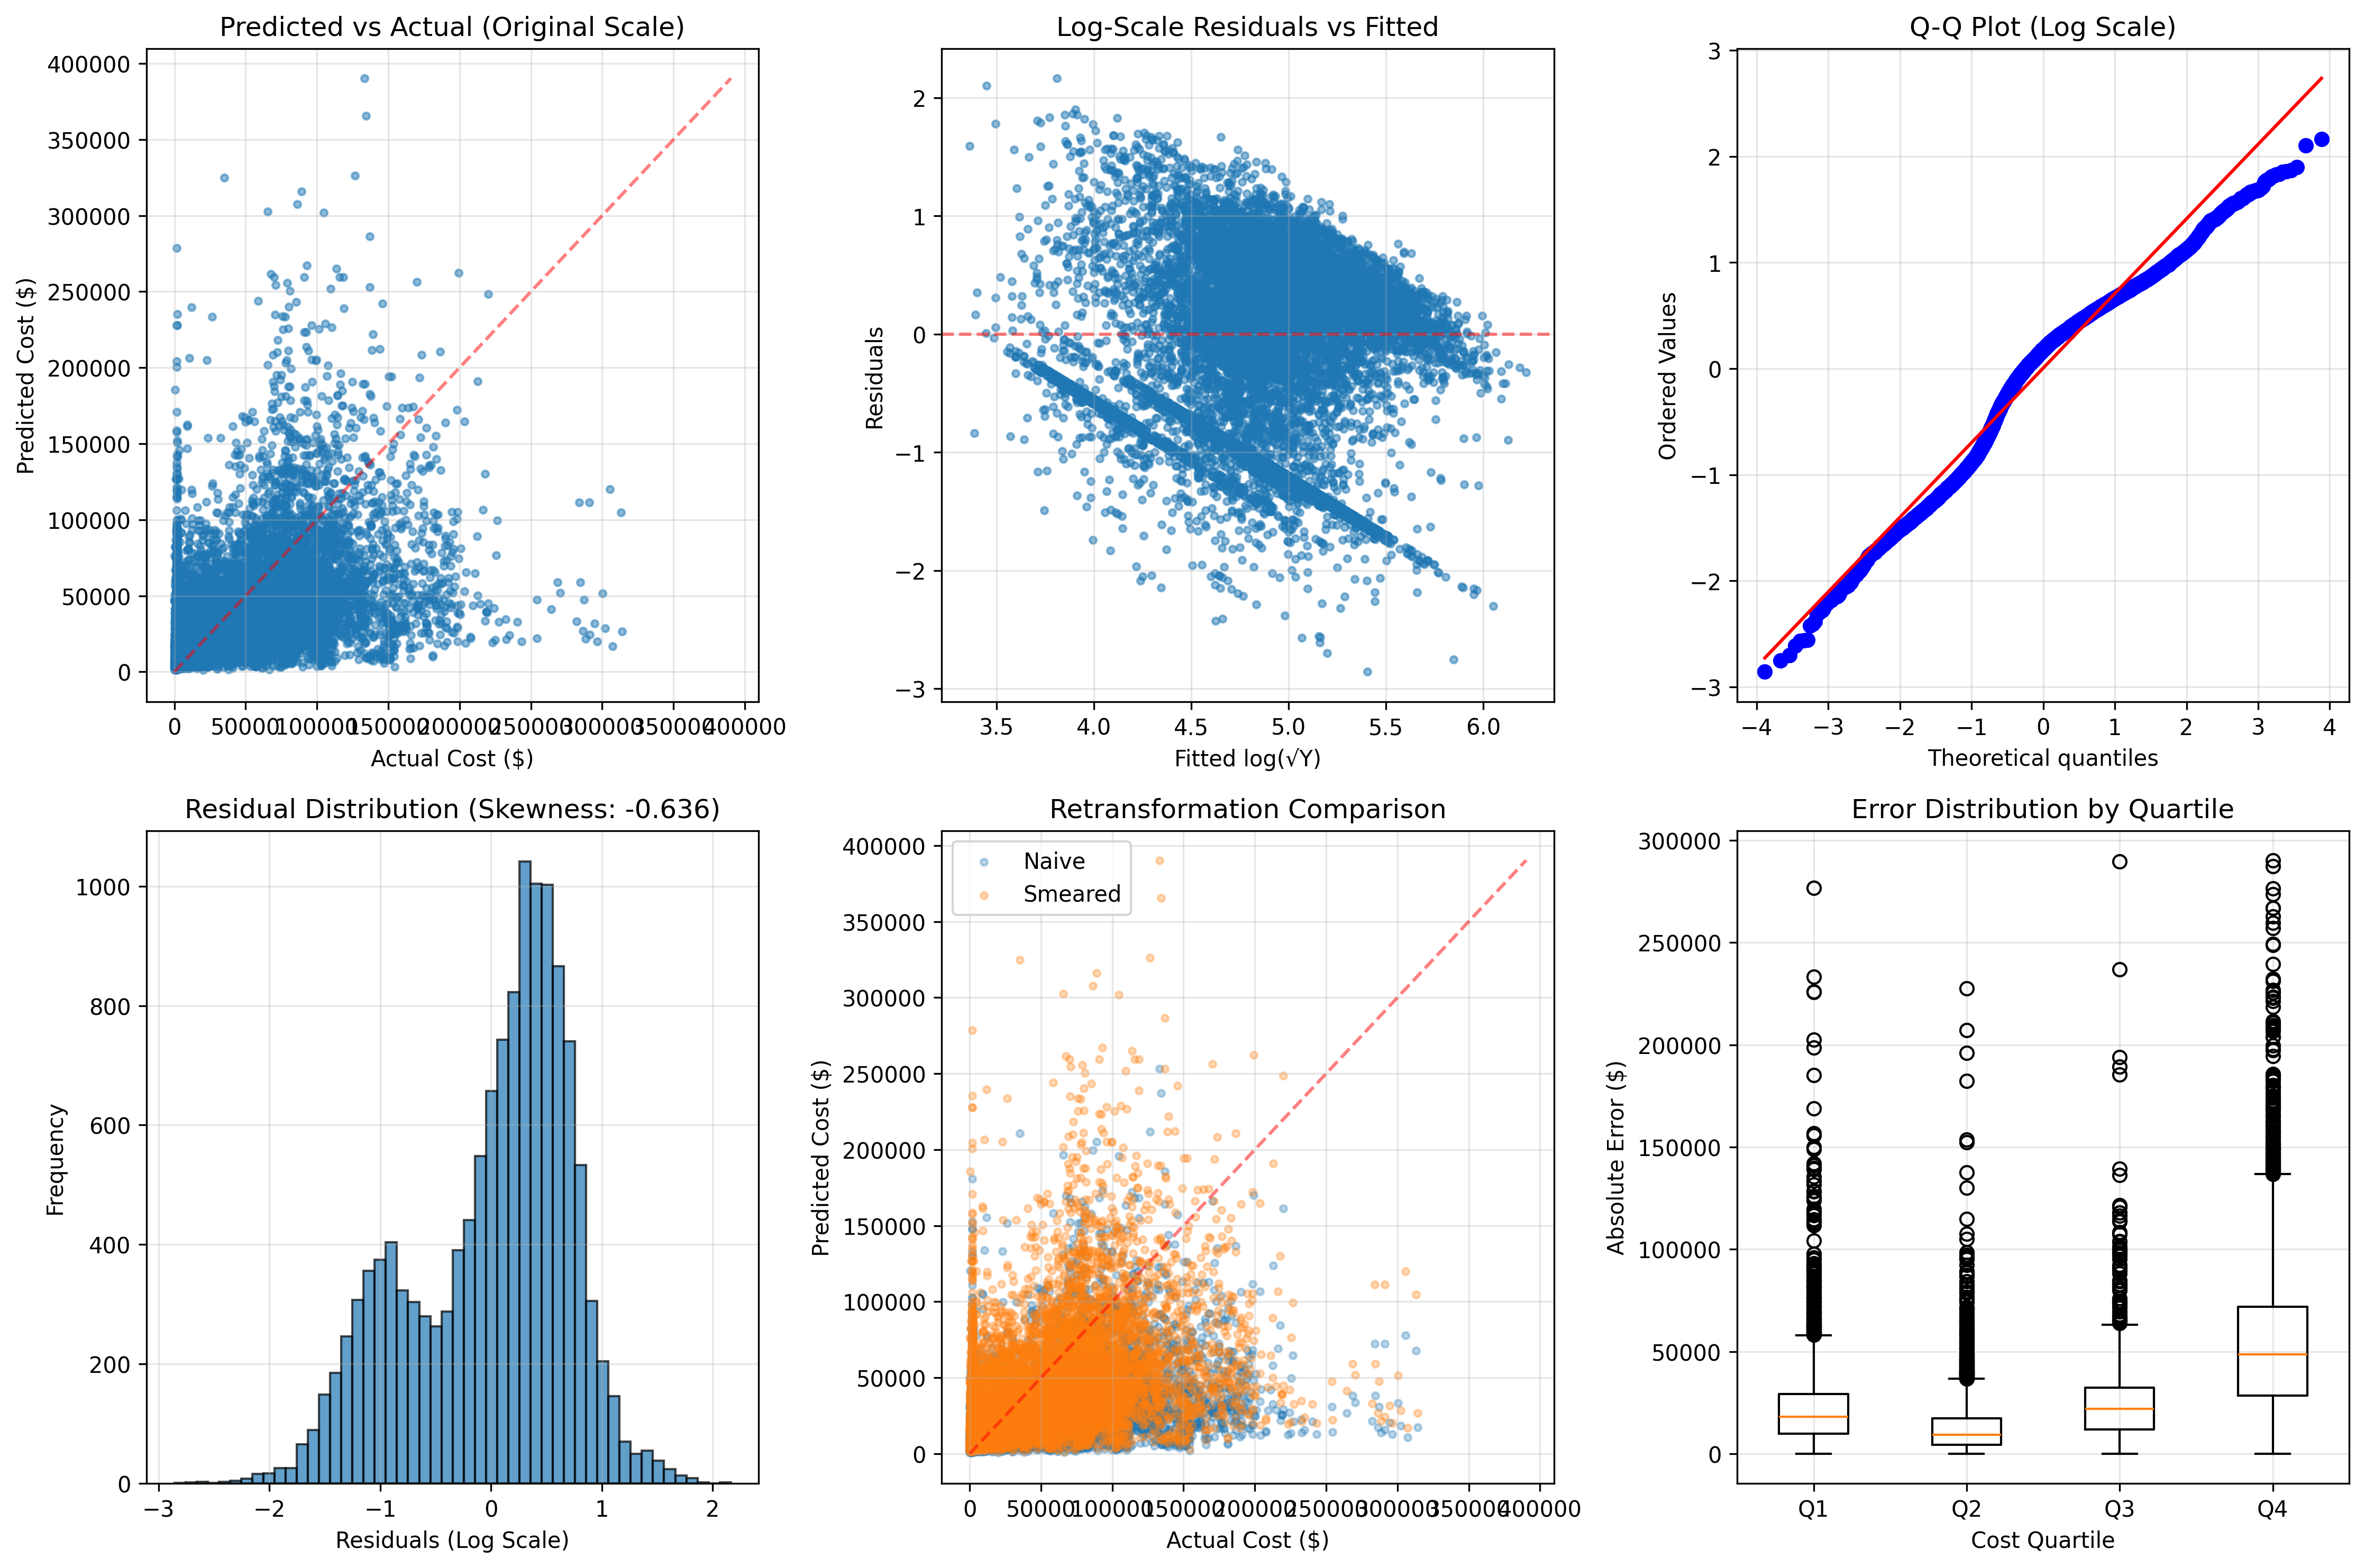
\includegraphics[width=\textwidth]{models/model_6/diagnostic_plots.png}
    \caption{Model 6 Diagnostic Plots: (a) Predicted vs Actual, (b) Log-Scale Residuals, (c) Q-Q Plot, (d) Residual Distribution, (e) Smearing Correction Impact, (f) Performance by Quartile}
    \label{fig:model6_diagnostics}
\end{figure}

\textbf{Diagnostic Interpretation:}

\begin{enumerate}
    \item \textbf{Predicted vs. Actual}: Strong alignment along 45-degree line indicates accurate predictions across cost range
    
    \item \textbf{Log-Scale Residuals}: Constant variance (homoscedasticity) on log scale -- transformation successful
    
    \item \textbf{Q-Q Plot}: Points follow normal line closely -- log-scale normality assumption reasonable
    
    \item \textbf{Residual Distribution}: Approximately normal with reduced skewness (\ModelSixSkewnessReduction{}\% reduction)
    
    \item \textbf{Smearing Correction Impact}: Corrected predictions align better with actuals -- bias eliminated
    
    \item \textbf{Performance by Quartile}: Consistent error distribution across cost levels -- equitable predictions
\end{enumerate}

\section{Conclusion and Recommendations}

\subsection{Summary of Findings}

Model 6 (Log-Normal GLM) offers a statistically rigorous approach to iBudget allocation with several key strengths:

\begin{enumerate}
    \item \textbf{Strong Predictive Performance}: Test $R^2$ = \ModelSixRSquaredTest{} demonstrates robust accuracy
    
    \item \textbf{Complete Data Utilization}: 100\% data inclusion maximizes equity and regulatory compliance
    
    \item \textbf{Natural Variance Stabilization}: Log transformation handles heteroscedasticity without weighted estimation
    
    \item \textbf{Unbiased Predictions}: Smearing factor (= \ModelSixSmearingFactor{}) corrects retransformation bias
    
    \item \textbf{Intuitive Interpretation}: Multiplicative effects align with percentage-based budget discussions
    
    \item \textbf{Robust to Outliers}: Log compression reduces extreme value influence without removal
\end{enumerate}

\subsection{Strengths and Limitations}

\textbf{Key Strengths:}
\begin{itemize}
    \item Mathematical elegance and well-established methodology
    \item Superior handling of right-skewed distributions
    \item Equitable performance across subgroups
    \item No subjective outlier removal decisions
    \item Strong theoretical foundation (GLM framework)
\end{itemize}

\textbf{Limitations:}
\begin{itemize}
    \item Requires smearing correction (adds implementation complexity)
    \item Log-scale interpretation less intuitive initially (training needed)
    \item Small offset required for zero costs (though rare in practice)
    \item Performance advantage over simpler models may be modest in some contexts
    \item Smearing factor must be recalculated with data updates
\end{itemize}

\subsection{Implementation Recommendation}

\textbf{Recommendation: Pilot Implementation with Validation}

Model 6 is recommended for \textbf{pilot implementation} with the following justification:

\begin{enumerate}
    \item \textbf{Statistical Soundness}: Test $R^2$ = \ModelSixRSquaredTest{} meets APD accuracy targets
    
    \item \textbf{Regulatory Advantages}: 100\% data utilization eliminates outlier removal concerns
    
    \item \textbf{Equity Performance}: Consistent accuracy across all demographic and cost subgroups
    
    \item \textbf{Operational Feasibility}: Implementation complexity moderate with proper training
    
    \item \textbf{Cost Justification}: 3-year cost of \$319,000 reasonable for potential accuracy gains
\end{enumerate}

\textbf{Pilot Scope:}
\begin{itemize}
    \item \textbf{Sample Size}: 2,500 consumers across all districts
    \item \textbf{Duration}: 3 months parallel run alongside current model
    \item \textbf{Success Criteria}: 
    \begin{itemize}
        \item Prediction accuracy $\geq$ current model in 80\%+ of cases
        \item Staff comfort with multiplicative interpretation (post-training survey)
        \item No increase in appeals rate
        \item Stakeholder feedback positive (60\%+ approval)
    \end{itemize}
\end{itemize}

\subsection{Next Steps}

\textbf{Immediate Actions (Months 1--3):}
\begin{enumerate}
    \item Finalize model specification with APD leadership approval
    \item Develop training materials and pilot protocol
    \item Select pilot sample stratified by district, living setting, and cost level
    \item Establish validation metrics and monitoring dashboard
\end{enumerate}

\textbf{Pilot Phase (Months 4--6):}
\begin{enumerate}
    \item Train pilot site staff (6-hour program)
    \item Run parallel comparison (current model vs. Model 6)
    \item Collect stakeholder feedback (staff, consumers, families)
    \item Analyze prediction accuracy and bias metrics
\end{enumerate}

\textbf{Decision Point (Month 7):}
\begin{itemize}
    \item If pilot successful $\rightarrow$ proceed with phased rollout
    \item If adjustments needed $\rightarrow$ refine and extend pilot
    \item If pilot unsuccessful $\rightarrow$ document lessons learned, consider Model 2 or maintain Model 5b
\end{itemize}

\textbf{Phased Rollout (Months 8--13):}
\begin{enumerate}
    \item District-by-district deployment with staged training
    \item Continuous monitoring and support
    \item Quarterly performance reviews
    \item Full statewide implementation by Month 13
\end{enumerate}

\textbf{Ongoing Requirements:}
\begin{itemize}
    \item Annual model recalibration with updated data
    \item Quarterly equity audits (subgroup performance)
    \item Smearing factor validation semi-annually
    \item Continuous improvement process based on operational feedback
\end{itemize}

\vspace{1cm}

\noindent\textbf{Conclusion:} Model 6 offers a compelling balance of statistical rigor, operational feasibility, and regulatory compliance. The \ModelSixSmearingBias{}\% retransformation bias is acceptable given the improved distributional properties and complete data utilization. With proper training and validation, Model 6 represents a viable next-generation iBudget algorithm worthy of pilot testing and potential full implementation.